\subsection{Introduction}
Spike trains can be analyzed by exploiting several kinds of techniques, according
to the aim of the analysis. In particular, it might be interesting to study the
behaviour of a recording site after an external stimulation. Notice that this kind
of analysis becomes more and more relevant as it is extended to multiple channels, for
instance in order to study how different neurons react to the same stimulus.
Alternatively, the responses from several subjects can be compared as well. Other
interesting analyses might consist in comparing several channels or corresponding
channels in different subjects, establishing proper metrics to assess similarity
and correlation.

\subsection{Post Stimulus Time Histogram}
Post Stimulus Time Histogram (PSTH) is a vital tool to characterize neural spike trains
in response to a stimulus. Notice that in general the response of a certain neuron
for a repeated given stimulus is not identical, but it tends to change, as in the
adaptation phenomenon.\\
The intensity of the response and its dynamics is visualized through an histogram.
As a matter of fact, a certain time window is isolated after the occurrence of the
stimulus and it is divided into several equally long bins. Then, the total number of
spikes in each bin is counted and reported into the histogram, as shown in the figure
below.
\begin{figure}[H]
    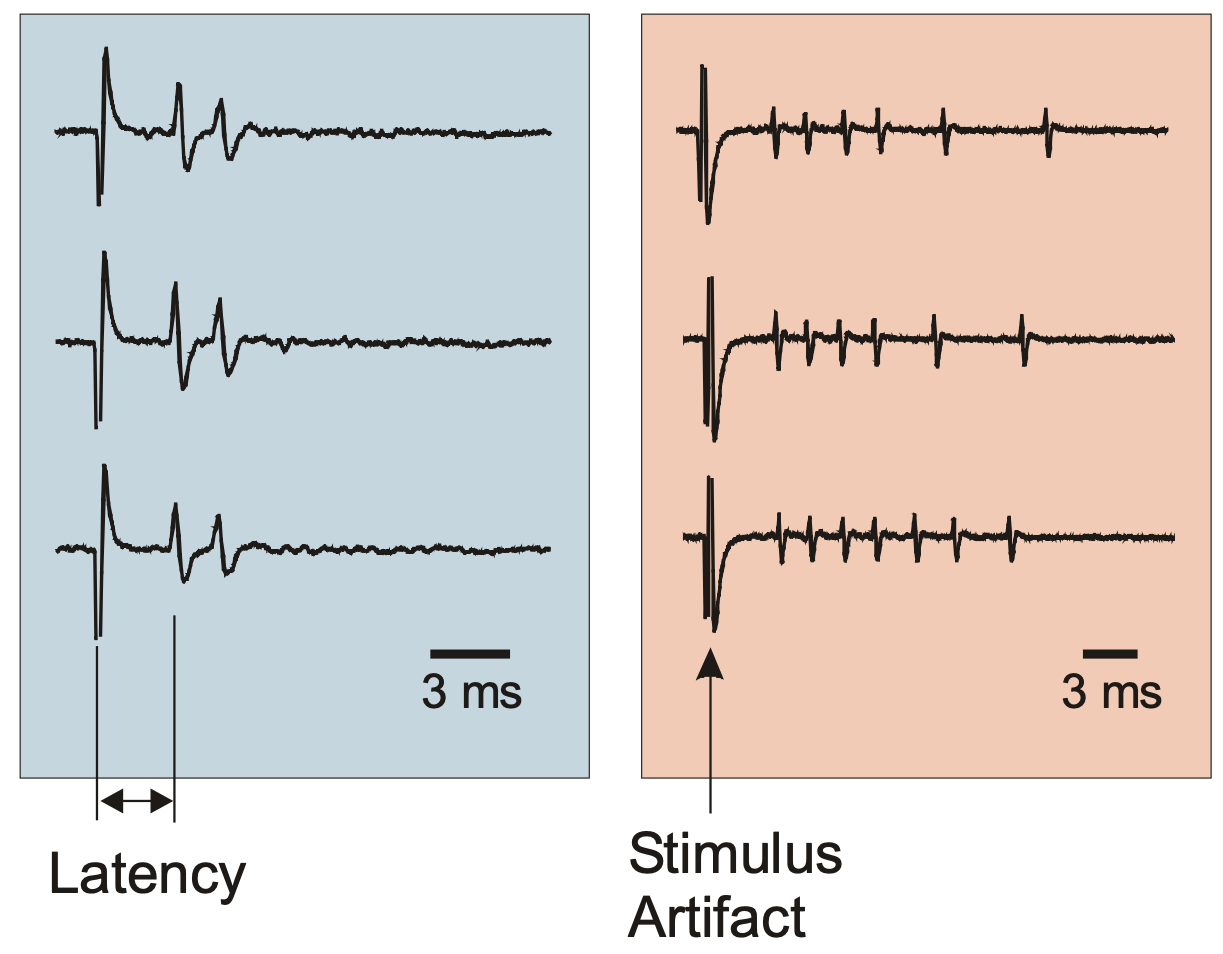
\includegraphics[scale=0.75]{8_1}
    \centering
\end{figure}
Notice that the spike count can be normalized in order to obtain the firing rate, which
can be interpreted also as the probability of firing per time unit.\\
As already state, it is possible to derive several distinct kinds of PSTH, according to
the use case. It can be computed for a single neuron or a single recording site. It
can be computed distinctly for each site of a multi-channel recording, generating
a large number of PST histograms. On the other hand, an averaged PSTH is commonly used
to asses the average response of a network with several recording sites. Nonetheless,
an average PSTH is also employed to consider together spike trains generated in
multiple trials or subjects.
\begin{figure}[H]
    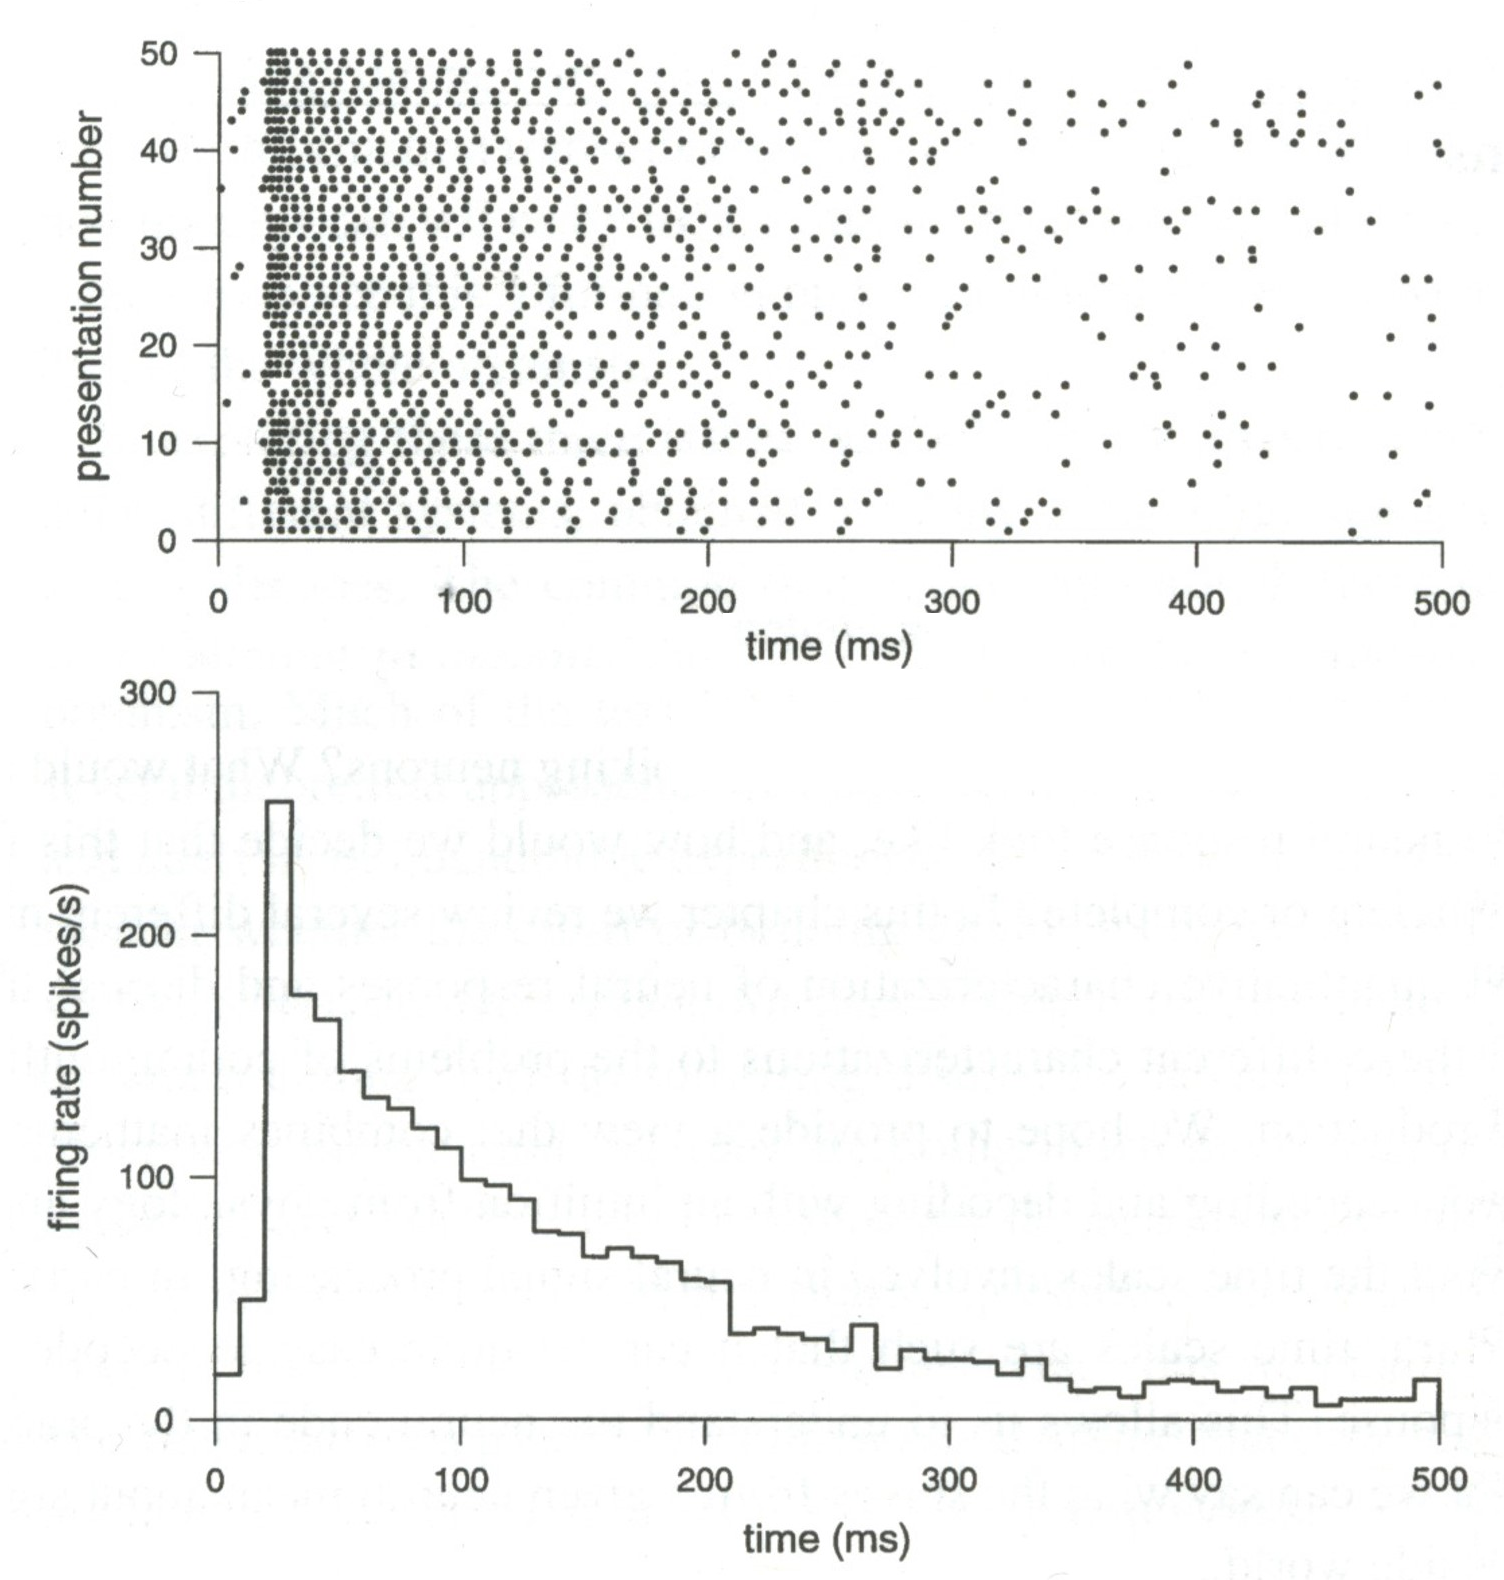
\includegraphics[scale=0.3]{8_2}
    \centering
\end{figure}
Generally, after after being stimulated, a neuron exhibits two different responses:
\begin{itemize}
    \item \textbf{Early response:} it occurs in the first \(50\,ms\) after the stimulus
          and includes the direct activation of the neuron.
    \item \textbf{Late (or delayed) response:} it occurs at least after \(50\,ms\) and up to
          \(400\,ms\), representing a reverberating response.
\end{itemize}
It can be said that the early response is definitely more reliable than the late
response, as the second one might be influenced by noise. A way to better focus
on the early response direct activation consists in chemically blocking the synapses.
\begin{figure}[H]
    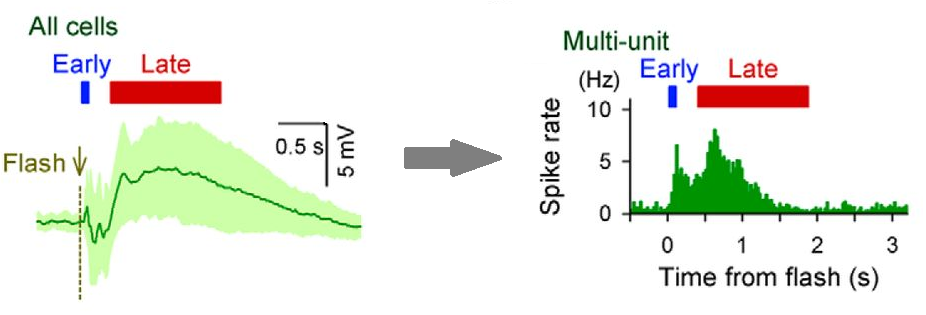
\includegraphics[scale=1.75]{8_3}
    \centering
\end{figure}
In addition, PST histograms might represent a valuable tool to individuate Major Burst
Leaders (MBLs), as they highlight the rapidity of a neuron to produce a response. In the
following picture a PSTH for each channel of an array of electrodes is represented,
according to the physical layout of the electrodes, and the MBLs are highlighted in red.
\begin{figure}[H]
    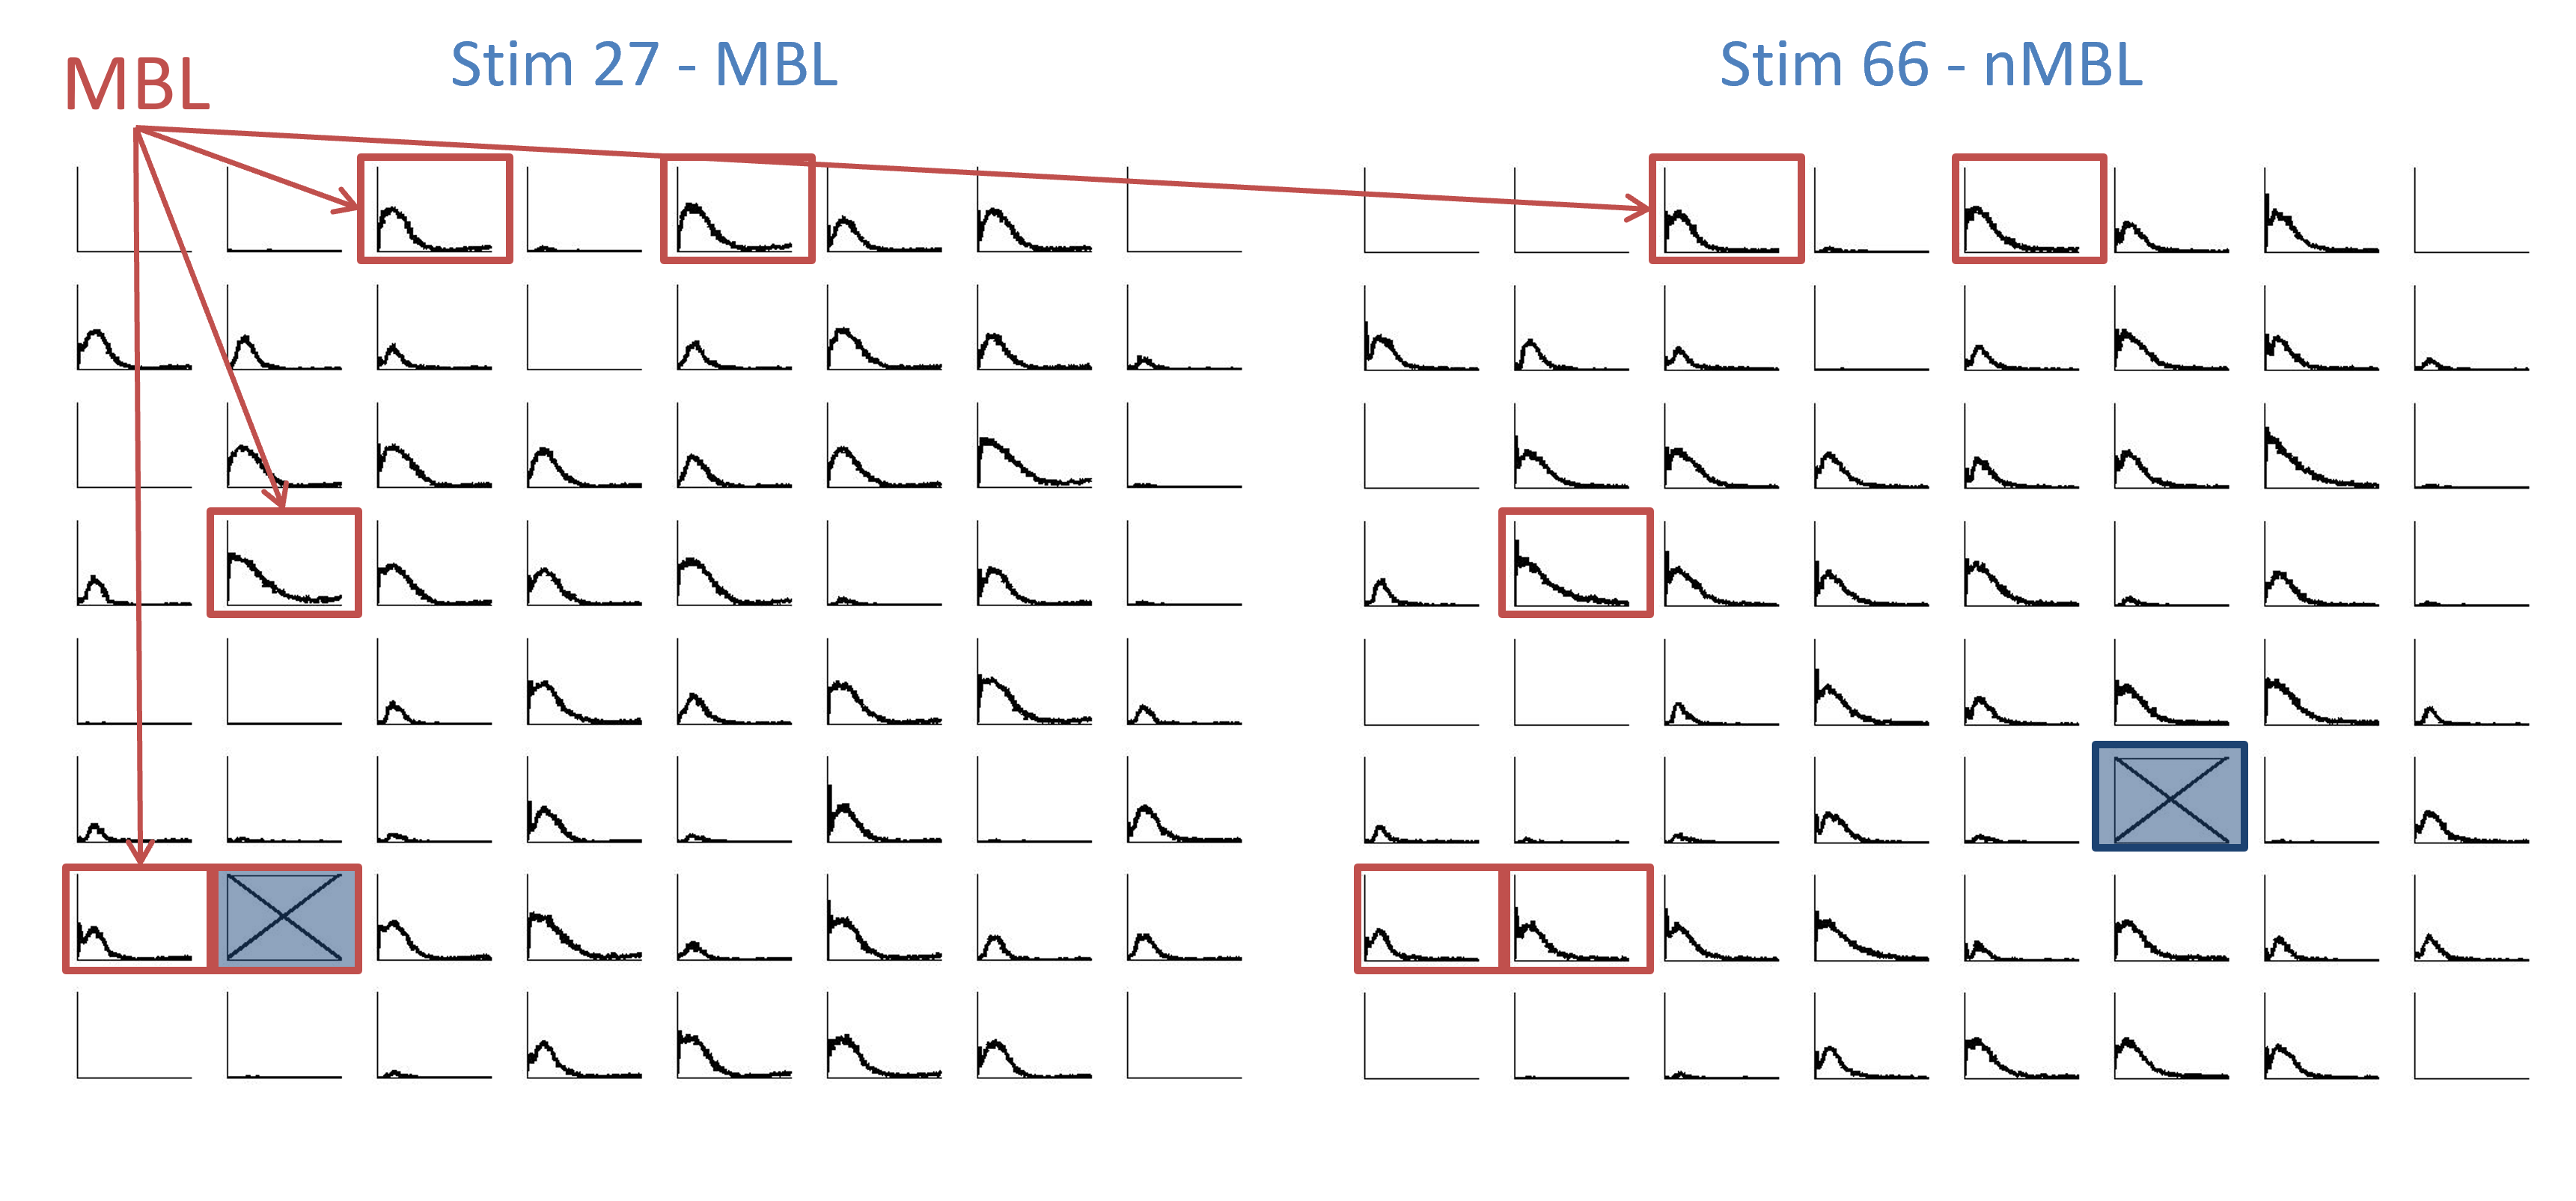
\includegraphics[scale=0.6]{8_4}
    \centering
\end{figure}

\subsection{Cross-Correlation}
The cross-correlation between spike trains is a fundamental metric, as it is capable
to highlight synchronization phenomena at the network level. Notice that this metric
can alternatively be computed starting from the spike trains or the burst trains.
A train is defined as the reference train, identified by \(x\), while the other
one is employed as the target train, denoted by \(y\).\\
The two trains are divided into equally spaced bins small enough to contain at most
one spike, then a cross-correlogram - i.e. a cross-correlation histogram - is derived
by counting the number of bins displaying a spike in both the reference and the target
trains. A time delay \(\tau\) is applied as a variable shift between the two trains.
Notice that by switching the reverse and the target trains, the same plot is obtained,
but reversed in the horizontal time axis.
\begin{figure}[H]
    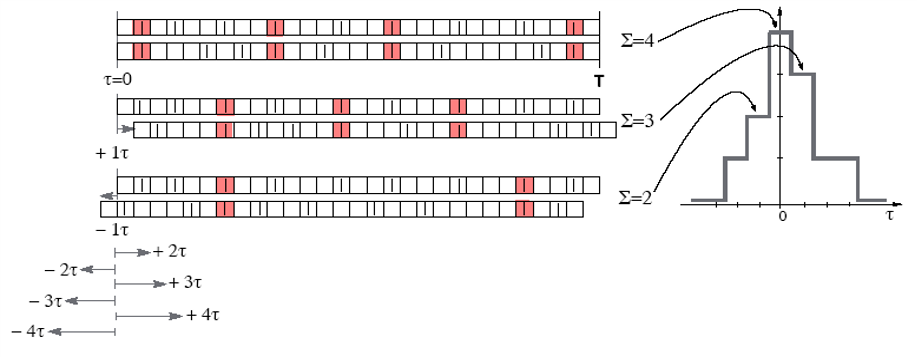
\includegraphics[scale=0.9]{8_5}
    \centering
\end{figure}
From a mathematical point of view, the cross-correlation \(C_{xy}\) can be formalized
as follow:
\begin{align*}
    C_{xy}(\tau)
    =\sum_{s=1}^{N_x}\sum_{t_{i}=(\tau-\Delta{\tau}/2)}^{(\tau+\Delta{\tau}/2)}x(t_s)y(t_s-t_i)
\end{align*}
Notice that a normalization term can be easily added in order to provide
a cross-correlation value in the \([0, 1]\) range:
\begin{align*}
    C_{xy}(\tau)
    =\frac{1}{\sqrt{N_xN_y}}\sum_{s=1}^{N_x}\sum_{t_{i}=(\tau-\Delta{\tau}/2)}^{(\tau+\Delta{\tau}/2)}x(t_s)y(t_s-t_i)
\end{align*}
where \(N_x\) is the total number of spikes in the reference train and \(N_y\) is the
total number of spikes in the target train. The previously described properties of
\(C_{xy}(\tau)\) can be summarized as follow:
\begin{itemize}
    \item \(0\le{C_{xy}(\tau)}\le{1}\)
    \item \(C_{xy}(\tau)=C_{yx}(-\tau)\)
\end{itemize}
Auto-correlation is often used to test the functioning of a cross-correlation
algorithm:
\begin{align*}
    C_{xx}(\tau)
     & =\frac{1}{\sqrt{N_xN_x}}\sum_{s=1}^{N_x}\sum_{t_{i}=(\tau-\Delta{\tau}/2)}^{(\tau+\Delta{\tau}/2)}x(t_s)x(t_s-t_i) \\
     & =\frac{1}{N_x}\sum_{s=1}^{N_x}\sum_{t_{i}=(\tau-\Delta{\tau}/2)}^{(\tau+\Delta{\tau}/2)}x(t_s)x(t_s-t_i)
\end{align*}
\begin{figure}[H]
    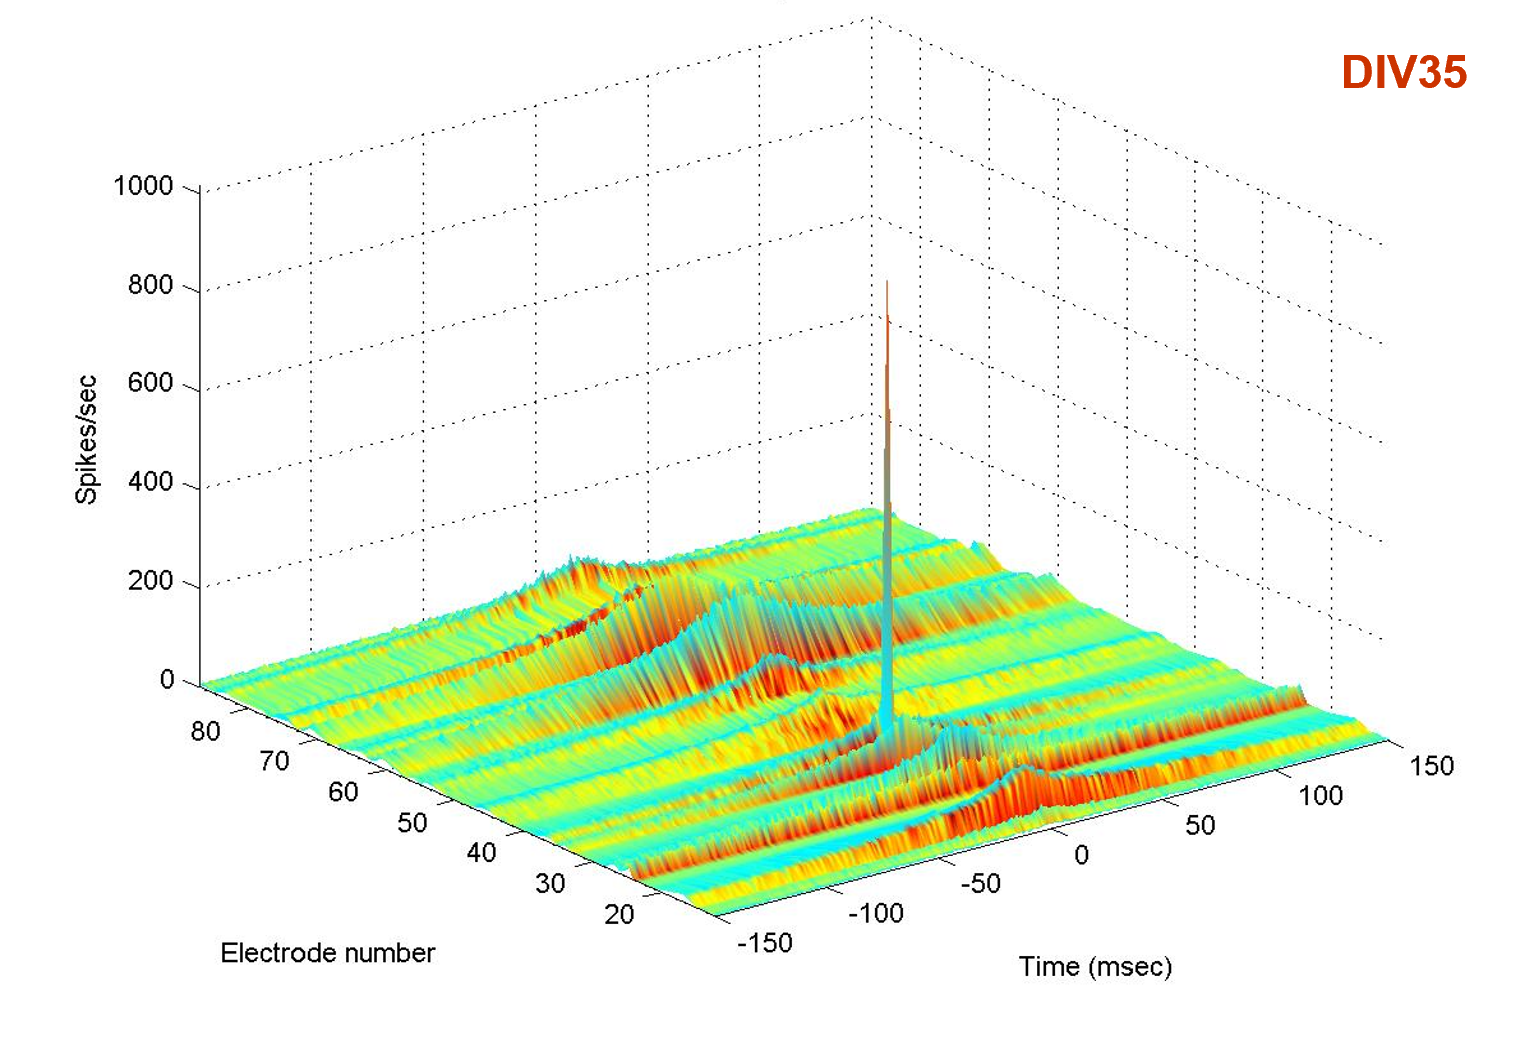
\includegraphics[scale=0.9]{8_6}
    \centering
\end{figure}
A further mean-correlogram can be computed to assess how one channel is correlated
to all of the others:
\begin{align*}
    C_x(\tau)=\frac{1}{n-1}\sum_{y=1}^{n}C_{xy}(\tau)
\end{align*}
It is now possible to define the cross-correlation function in zero \(C(0)\), with
the bin centered in zero:
\begin{align*}
    C(0)=\sum_{\tau=-k(\Delta\tau/2)}^{k(\Delta\tau/2)}C_{xy}(\tau)
\end{align*}
with \(\Delta\tau\) being the bin size and \(k\) indicating the considered number of
bin around the central one, identified as bin zero.
On the other hand, the \(C_{peak}\) represents the value of the cross-correlogram in
an area around the maximum detected peak. This is computed in order to quantify the
correlation level among all the recording channels. The peak latency is the distance
of the maximum peak from the zero: it can be interpreted as the delay of an
estimated functional connection.
\begin{align*}
    C_{peak}=\sum_{\tau=\tau_{peak}-k(\Delta\tau/2)}^{\tau_{peak}+k(\Delta\tau/2)}C_{xy}(\tau)
\end{align*}
Two channels can be considered to be synchronized whenever the central peak is
centered in zero, implying a very small peak latency.
\begin{figure}[H]
    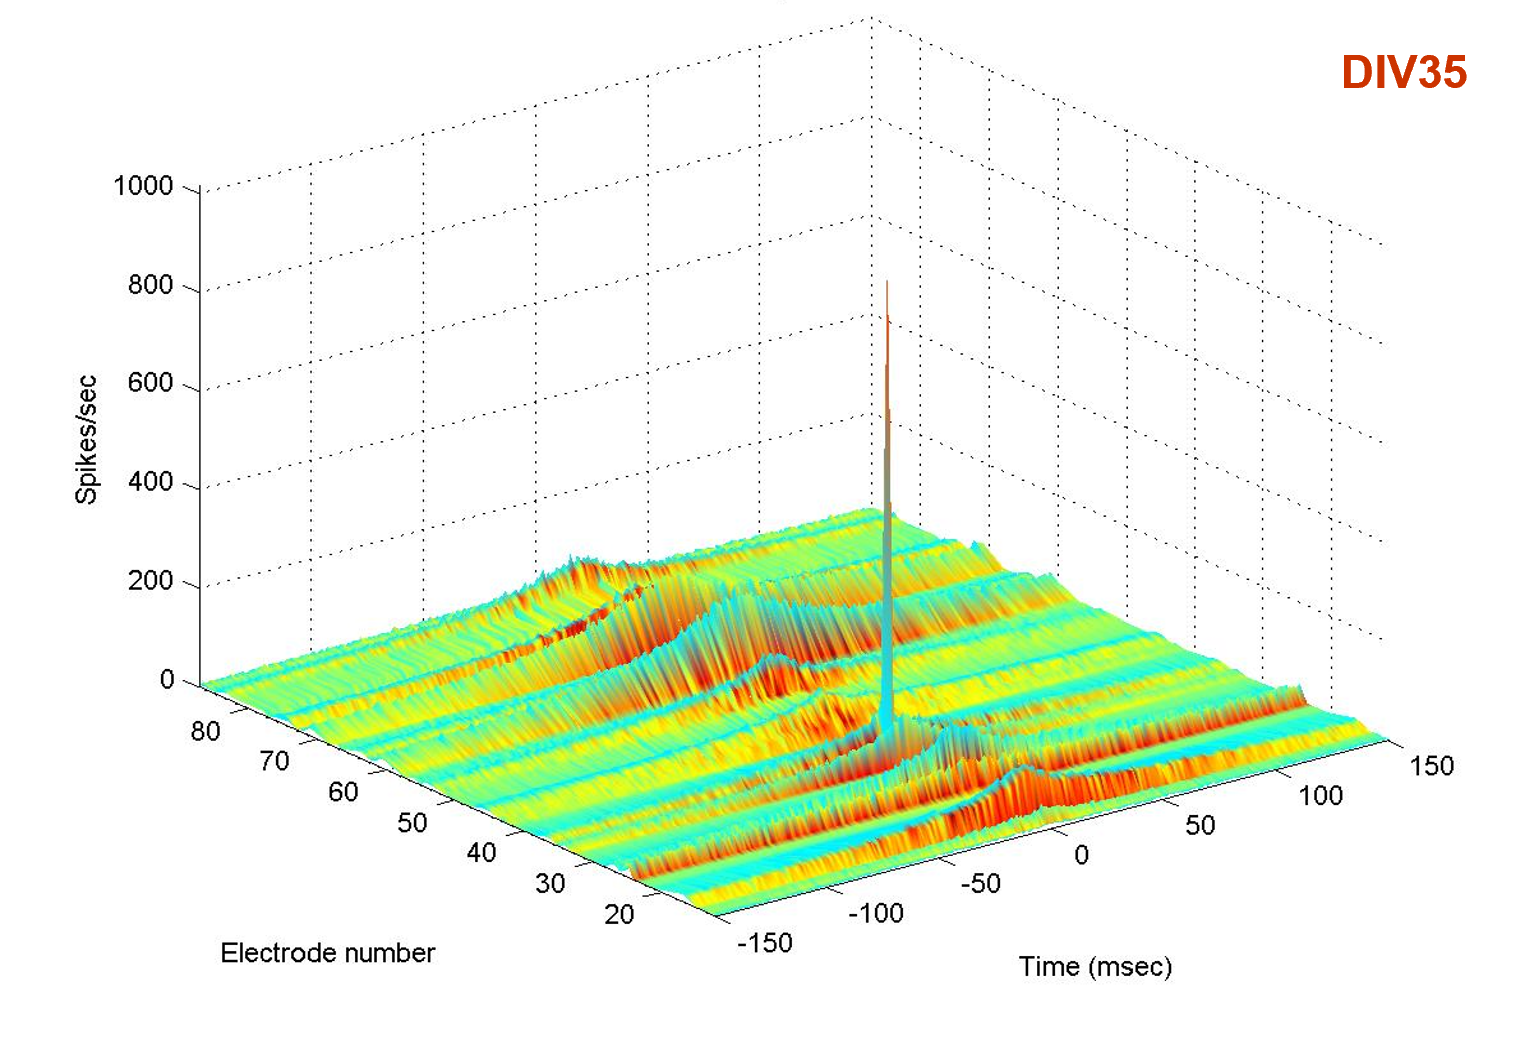
\includegraphics[scale=0.9]{8_7}
    \centering
\end{figure}

\subsubsection{The Coincidence Index}
The Coincidence Index, often indicated with \(CI\), is a percentage indicator of the
synchronization level between two channels. It can be defined both for 0 and for
the correlation peak.
\begin{align*}
    CI_{zero} & = \frac{C(0)}{\sum_{\tau=-T}^{T}C_{xy}(\tau)}     \\
    CI_{peak} & = \frac{C_{peak}}{\sum_{\tau=-T}^{T}C_{xy}(\tau)}
\end{align*}
Notice that the denominator \(\sum_{\tau=-T}^{T}C_{xy}(\tau)\) represents the total
area under the cross-correlogram curve.

\subsubsection{The Pearson's Correlation Coefficient}
This metric is widely used to indicate the correlation between two variables \(X\)
and \(Y\) - i.e. the degree to which the variables are related to each other.
When computed in a sample, the Pearson's Correlation Coefficient is indicated as \(r\).
Notice that it reflects the degree of linear relationship between two variables,
in the \([-1;+1]\) range:
\begin{itemize}
    \item \(\mathbf{r=+1}\): there is a \textbf{perfect positive linear
              relationship} between the variables \(X\) and \(Y\Rightarrow\) high scores on
          the X-axis are associated with high scores on the Y-axis.
    \item \(\mathbf{r=-1}\): there is a \textbf{perfect negative linear
              relationship} between the variables \(X\) and \(Y\Rightarrow\) high scores on
          the X-axis are associated with low scores on the Y-axis.
    \item \(\mathbf{r=0}\): there is \textbf{no linear
              relationship} between the variables \(X\) and \(Y\).
\end{itemize}
Generally, the Pearson's Correlation Coefficient is computed as follow:
\begin{align*}
    r=\frac{\sum_{i=1}^{N}(x_i-\overline{x})(y_i-\overline{y})}{\sqrt{\sum_{i=1}^{N}(x_i-\overline{x})^2\sum_{i=1}^{N}(y_i-\overline{y})^2}}
\end{align*}
In the neuroscience field, the Pearson's Correlation Coefficient has been preoposed
as a measure of synchronization among different units of a neuronal network.
In this case, \(r\) can be computed in a much easier way:
\begin{align*}
    r=\frac{N\sum_{i=1}^{N}x_{i}y_{i}-N_{x}N_{y}}{\sqrt{N_{x}(N-N_{x})}\sqrt{N_{y}(N-N_{y})}}
\end{align*}

\subsubsection{Visualization Tools}
Various graphic tools can be employed to visualize the correlation degree of several
recording channels in a neuronal network.
\paragraph{Multi-Channel Raster Plot} This kind of plots allows the visual inspection
of several channels at the same time, making easy to see if the spike trains coming
from different recording sites are similar to one another. Although this tool is
pretty simple to employ, it becomes ineffective in the case of correlations that are
not immediately visible.
\begin{figure}[H]
    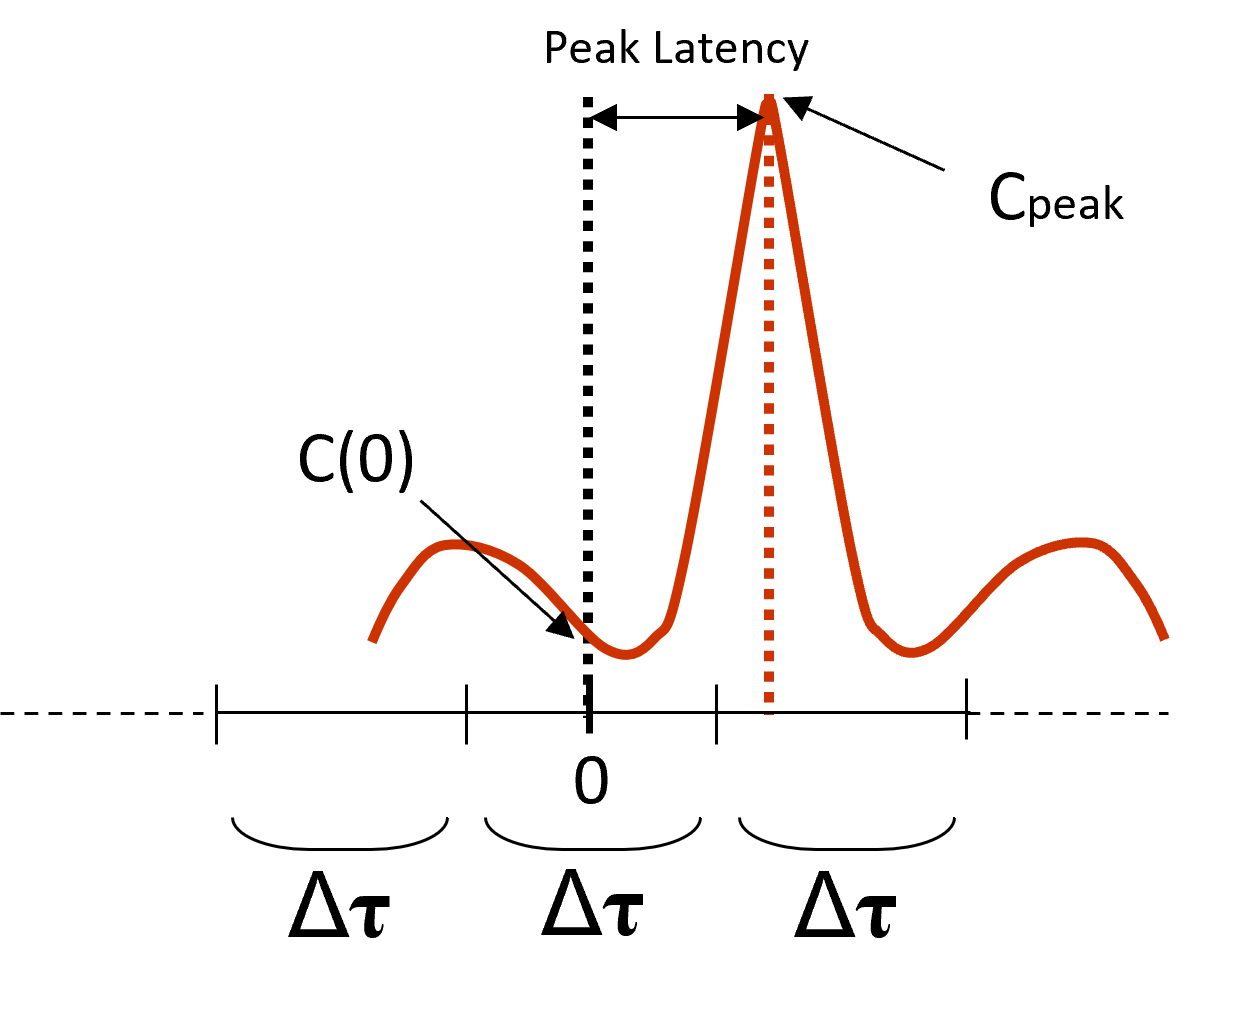
\includegraphics[scale=0.78]{8_8}
    \centering
\end{figure}
\paragraph{Correlation Matrix Plot} The correlation matrix is usually computed for
the zero point, thus it is indicated as \(C(0)\), and for every possible pair of
recording channels. The values are then plotted by using a heatmap. Notice that the
main diagonal exhibits a maximum correlation, as it represents the auto-correlation
for each channel.
\begin{figure}[H]
    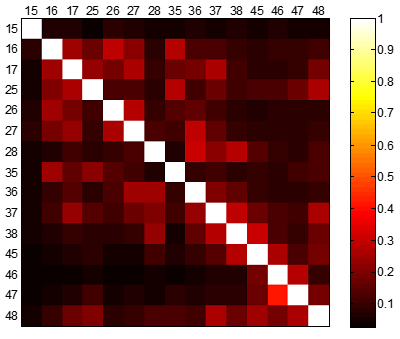
\includegraphics[scale=0.8]{8_9}
    \centering
\end{figure}
\paragraph{Connectivity Map} This method allows to plot a topological mapping of the
connections between the sources, according to their activity. Each node is drawn,
according to its position on the MUA. Then, the correlation \(C(0)\) between each pair
of the recording channels is computed and a connecting line is added if \(C(0)\)
overcomes an arbitrary threshold - i.e. \(C(0)>0.2\). In addition, the thickness of
the line is made proportial to the degree of correlation between the two nodes.
Notice that it is common to observe stronger connections between nodes close to
each other.
\begin{figure}[H]
    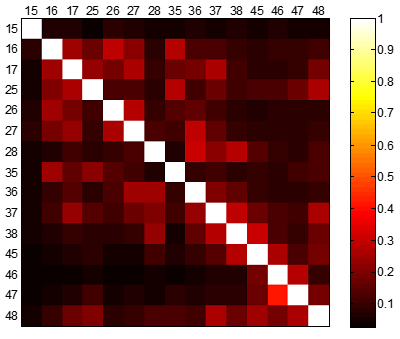
\includegraphics[scale=1.2]{8_10}
    \centering
\end{figure}